\documentclass{article}
\usepackage{graphicx}
\usepackage[utf8]{inputenc}
\usepackage{fullpage}
\usepackage{enumitem}
\usepackage{hyperref}
\usepackage{titling}
\usepackage{mathtools}

\parindent0in
\pagestyle{plain}
\thispagestyle{plain}

\newcommand{\myname}{John Doe}
\newcommand{\assignment}{Práctica SVM}
\newcommand{\duedate}{27 de Noviembre, 2018}

\renewcommand\thesubsection{\arabic{subsection}}

\title{Support Vector Machine}
\date{}

\begin{document}

Universidad Católica San Pablo\hfill\\
Sistemas Inteligentes\hfill\textbf{\assignment}\\
Prof.\ José Ochoa, Graciela Mesa\hfill\textbf{Entrega:} \duedate\\
\smallskip\hrule\bigskip

{\let\newpage\relax\maketitle}
% \maketitle

\section{Preguntas de Teoría:}
Sea el conjunto $S = \{((1, 6), -1), ((4, 9), -1),((4, 6), -1), ((5, 1), 1), ((9,5), 1), ((9,1), 1)\}$ y un conjunto de cuatro
hiperplanos $H = \{H_1, H_2, H_3, H_4\}$, definidos como: $H_1: x1 - x2 - 1 = 0$, $H_2: 2x1 - 7x2 +32 = 0$,
$H_3: \sqrt{\frac{1}{2}}x1 - \sqrt{\frac{1}{2}}x2 - \sqrt{\frac{1}{2}} = 0$, $H_4: 2x1 - 7x2  - 32 = 0$

\begin{enumerate}
    \item Usando cualquier lenguaje de programación grafique $S$, $H_1$, $H_2$, $H_3$ y $H_4$
    
    Código escrito en python utilizando la libreria $Matplotlib$. Ver Fig.$\ref{CODE_P1_1}$
    \begin{figure}[h]
            \label{CODE_P1_1}
            \centering
            \includegraphics[width=.6\textwidth]{code_1_1.png}
            \caption{Código ploteo Puntos e hiperplanos}
    \end{figure}

    Resultado del programa. Ver Fig. $\ref{PLOT_P1_1}$:
    \begin{figure}[h]
        \label{PLOT_P1_1}
        \centering
        \includegraphics[width=.6\textwidth]{Figure_1_1.png}
        \caption{Puntos e hiperplanos, conjunto separable}
    \end{figure}

    \item Encuentre los parametros \textbf{w, b} que definen los hiperplanos
    $\{H_1, H_2, H_3, H_4\}$ y luego determine para $\{H_1, H_2, H_3, H_4\}$ si son hiperplanos de separación.
    Fundamente.

    Ya que son hiperplanos, estos cumplen lo siguiente:
    \[
        < {w}, {x_i}> + b = 0  
    \]
    Para ver si son planos de separación debe cumplir con la siguiente definición: Una función
    lineal que es capaz de separar dicho conjunto sin error.

    Para $H_1: x1 - x2 - 1 = 0$, por tanto $w1 = 1, w2 = -1, b = -1$
    
    Ya que es una función lineal y además separa el conjunto sin error, se puede considerar este hiperplano 
    como un hiperplano de separación. Ver Fig. $\ref{PLOT_P1_1}$ \textit{curva azul}

    Para $H_2: 2x1 - 7x2 + 32 = 0$, por tanto $w1 = 2, w2 = -7, b = 32$
    Ya que es una función lineal y además separa el conjunto sin error, se puede considerar este hiperplano 
    como un hiperplano de separación. Ver Fig. $\ref{PLOT_P1_1}$ \textit{curva naranja}

    Para $H_3: \sqrt{\frac{1}{2}}x1 - \sqrt{\frac{1}{2}}x2 - \sqrt{\frac{1}{2}} = 0$, por tanto $w1 = \sqrt{\frac{1}{2}}, w2 = -\sqrt{\frac{1}{2}}, b = -\sqrt{\frac{1}{2}}$
    Ya que es una función lineal y además separa el conjunto sin error, se puede considerar este hiperplano 
    como un hiperplano de separación. Ver Fig. $\ref{PLOT_P1_1}$ \textit{curva azul}

    Para $H_4: 2x1 - 7x2 - 32 = 0$, por tanto $w1 = 2, w2 = -7, b = -32$

    En este caso el hiperplano $H_4$ no se considera de separación ya que los dos conjuntos se encuentran a un solo lado de la curva.
    Ver Fig. \ref{PLOT_P1_1} \textit{curva verde}

    \item En el conjunto $H$, ¿Cuántos hiperplanos iguales existen?. En el caso 
    de que existan, ¿Cuáles son estos?. Fundamente.

    Existen 2 hiperplanos iguales, que en las preguntas siguientes, son tratados como solo uno. Estos son $H_1$ y $H_3$, ya que
    el si se divide al hiperplano $H_3$ por una constante $\frac{1}{\sqrt{2}}$, el resultado es la ecuación matemática del 
    hiperplano $H_1$

    \item Calcule el margen $\tau$ para cada hiperplano de separación. Luego, suponga que el conjunto \textit{H}
    contiene al hiperplano óptimo, \textit{H}$^*$, ¿Cuál sería \textit{H}$^*$? Fundamente.

    Por geometría se sabe que la distancia entre un hiperplano de separación $D(x)$ y un
    ejemplo $x'$ viene dada por:
    \[
        \frac{\rvert D(x') \rvert}{\Vert \omega \Vert}   
    \]

    Siendo $D(x') = w_1*x_1 + w_2*x_2 + b$, para evitar calcular la distancia a cada punto, se utiliza la referencia gráfica \ref{PLOT_P1_1}
    Para \textbf{H1 y H3}:
    Distancia a la clase \textit{"-1"}: Punto $(4,6)$ y distancia a la clase \textit{"+1"}: Punto $(5, 1)$ y $(9, 5)$, en este caso
    se toma dos puntos, ya que gráficamente no se puede discriminar cual de los 2 esta más cerca.
    \[
        \tau(H_1) = min\{\frac{D_{H1}(4,6)}{\Vert \omega_{H1}\Vert}, \frac{D_{H1}(5,1)}{\Vert \omega_{H1}\Vert}, \frac{D_{H1}(9, 5)}{\Vert \omega_{H1}\Vert} \}    
    \]

    De la ecuación anterior se obtiene que:
    \[
        \tau(H_1) = \tau(H_3) = min\{\frac{3}{\sqrt{2}},\frac{3}{\sqrt{2}}, \frac{3}{\sqrt{2}}\} = \frac{3}{\sqrt{2}}
    \]
    Esto quiere decir que el punto más cercano a la hiperplano separador, para ambas categorías tienen la misma distancia.

    Para \textbf{H2}: 
    Distancia a la clase \textit{"-1"}: Punto $(4,6)$ y distancia a la clase \textit{"+1"}: Punto  y $(9, 5)$
    \[
        \tau(H_2) = min\{\frac{D_{H2}(4,6)}{\Vert \omega_{H2}\Vert}, \frac{D_{H2}(9, 5)}{\Vert \omega_{H2}\Vert} \}    
    \]

    De la ecuación anterior se obtiene que:
    \[
        \tau(H_2) = min\{0.27, 2.06\} = 0.27    
    \]

    Ya que \textbf{H4} no es un plano de separación, no tiene sentido calcular el valor de $\tau$.

    Suponiendo que el hiperplano óptimo se encuentra en el conjunto de hiperplanos definido lineas arriba, entonces este sería
    el hiperplano $H1$ ó $H3$, ya que este tendrá el margen máximo por estar a una distancia igual a cada clase. Esto se puede mostrar
    por reducción al absurdo.

    \item ¿Cuáles son los vectores de soporte del hiperplano \textit{H}$^*$ escogido en la pregunta anterior?, Fundamente.

    Para el caso anterior el vector de soporte estaría conformado por los puntos: $\{((4, 6), -1), ((5, 1), 1)\}$, ya que estos son
    los puntos más cercanos de cada clase al hiperplano separador.

    \item Demuestre la primera condición de \textnormal{KKT}, i.e: 
    \[
        \frac{\partial \mathcal{L}}{\partial w} (\omega^*, b^*, \alpha)= \omega^* - \sum_{i=1}^m \alpha_i y(i)x^{(i)}    
    \]
    
Sea el conjunto $N = \{((1, 6), -1), ((4, 9), -1),((4, 6), -1), ((5, 1), 1), ((9,5), 1), ((9,1), 1), ((0, 3), 1),$ \newline
$((2,2),-1), ((3,1),-1)\}$ y el
hiperplano $H_1$ definido anteriormente

    \item Usando cualquier lenguaje de programación grafíque $N$ y $H_5$

    \begin{figure}[h]
        \label{PLOT_P1_2}
        \centering
        \includegraphics[width=.6\textwidth]{Figure_2_N.png}
        \caption{Puntos e hiperplanos, cuasi separable}
    \end{figure}
    Ver Fig. $\ref{PLOT_P1_2}$. 

    \item Identifique los ejemplos que son separables y los que no lo son, luego, determine los ejemplos que son clasificados correctamente y los que no.

    Los ejemplos no separables se miden desde el borde que limíta su clase, es decir los que estan fuera de este límite. En este caso
    los ejemplos \textbf{no separables} son el siguiente conjunto de puntos: $M1 = \{((0, 3), 1), ((2,2),-1), ((3,1),-1) \}$, sin embargo el punto $(2,2)$ está
    bien clasificado.

    Ejemplos que si \textbf{son separables: } $N - M1$

    Ejemplos \textbf{mal clasificados} $M2 = \{((0, 3), 1),((3,1),-1)\}$

    Ejemplos \textbf{clasificados correctamente}: $N - M2$
    

    \item Calcule la holgura de los ejemplos no separables.

    Sean los ejemplos no separables y los puntos: $M1 = \{((0, 3), 1), ((2,2),-1), ((3,1),-1)\}$, y el hiperplano $H1$: $H_1: x1 - x2 - 1 = 0$
    Se define la $holgura \xi$:
    \[
        y_i(<\omega, x_i> + b) \geq 1 - \xi_i, \xi_i \geq 0, i = 1,\dots, n    
    \]

    Cálculo de $\xi_1$: $-4 \geq 1 - \xi_1$ $\Rightarrow \xi_1 = 5$

    Cálculo de $\xi_2$: $1 \geq 1 - \xi_2$ $\Rightarrow \xi_2 = 0$

    Cálculo de $\xi_3$: $-1 \geq 1 - \xi_3$ $\Rightarrow \xi_3 = 2$ 


    \section{Preguntas de Investigación}

    \item  Explique el significado de la constante $C$ en el término $C$ $\sum_{i=1}$ $\xi i$ que se qgrega ala función objetivo
    en el caso de ejemplos casi linealmente separables. Luego, explique la influencia de C en la capacidad de generalización de una $SVM$
    
    En el tutorial de \textit{Carmona-SVM}, pág. 8. menciona que la sumatoria de las holguras $\sum_{i=1}$ $\xi i$ es el coste asociado
    a los ejemplos no separables, así mismo multiplicar este término por una constante indicara que tanta importancia se le dará a este tipo de error.

    Darle un valor muy grande a la constante $C$ implica que se admita poco error $\sum \xi_i$, así mientras más grandes sea $C$, se considera a los ejemplos
    más separables.

    \item Describa el significado del parametro $\gamma$ en el kernel gaussiano. Luego, explique la influencia de $\gamma$ en la
    capacidad de generalización de una SVM.

    \section{Implementación}

    \item Usando el \textit{Scikit-learn} de \textit{Python}, implementar una $SVM$ que clasifique el conjunto un conjunto de datos.

    El código ha enviado en un $zip$.

    \item Experimente y muestre resultados usando diferentes valores para los parámetros de los kernels: lineal,
    polinomial, gaussiano, y el parámetro $C$.

    Resultado de clasificar con kernels \textit{lineal, polinomial y gaussiano}. Ver \ref{PLOT_P1_3}
    \begin{figure}[h]
        \label{PLOT_P1_3}
        \centering
        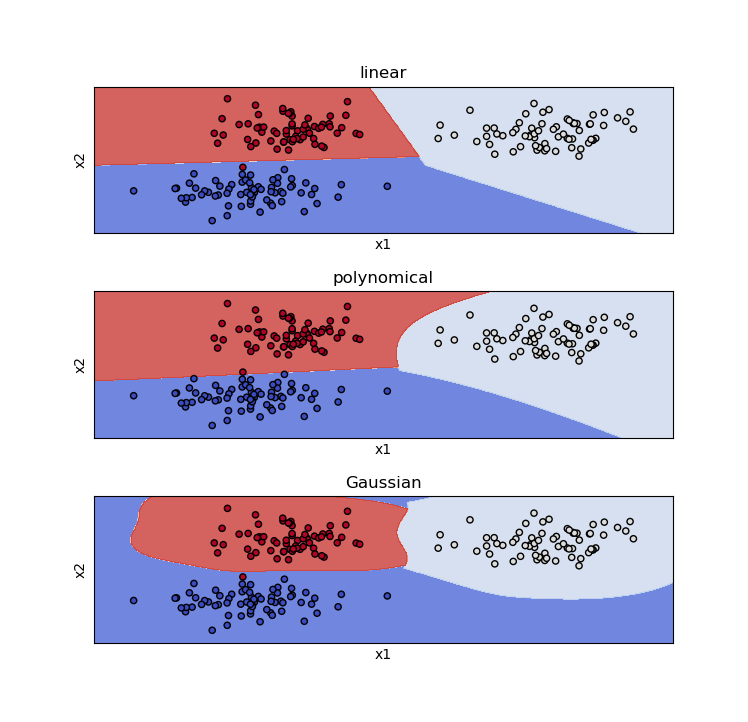
\includegraphics[width=.6\textwidth]{graphics_data1.png}
        \caption{C = 1.0}
    \end{figure}
     
    Resultado de clasificar con kernels \textit{lineal, polinomial y gaussiano}. Ver \ref{PLOT4}, para valores de $C$ bajos
    es decir con alta flexibilidad, se puede observar esto fuertemente en el kernel gaussiano.
    \begin{figure}[h]
        \label{PLOT4}
        \centering
        \includegraphics[width=.6\textwidth]{graphics_dataC.png}
        \caption{Lineal, Pol: C = 0.01, Gaussiano: C=0.03}
    \end{figure}

    \item Dentro de la sección de Implementación incluya una subsección donde indique las instrucciones
    para ejecutar su código.

    Leer el $Readme.md$

\end{enumerate}
\end{document}